\documentclass{article}
\usepackage{tbil-de}
%\usetikzlibrary{external}
%\tikzexternalize 
%\tikzsetexternalprefix{aux/}
\usepackage[top=1in,bottom=1in,right=1in,left=1in]{geometry}

\parindent=0pt
\parskip=1em

%Problem environment -- takes an argument which is the standard
\newenvironment{problem}[1]
%before
{
  \begin{flushleft}
  %{\bfseries \arabic{problem} .}
  %Problem numbering by standard
  \textbf{#1}.
  \ignorespaces
}
%after
{
  \end{flushleft}
}

\newenvironment{solution}
%before
{
  \ignorespaces
  \textbf{Solution:}
}
%after
{
  \ignorespacesafterend
  \begin{flushright}
  {\bfseries \qed}
  \end{flushright}
}



\begin{document}

\begin{center}
\Large \textbf{Sample Assessment Exercises}
\end{center}

This document contains one exercise and solution for each standard.
The goal is to give you an idea of what the exercises might look like,
and what the expectations for a complete solution are.



\begin{problem}{C1}
Find the general solution to \[y'+y=-t^2.\]
\end{problem}
\begin{solution}
First, we find a general solution to the homogeneous equation (removing all non-\(y\) terms) 
\[y_h'+y_h=0.\]
Since this is a first-order constant coefficient ODE, we know the answer is a modification of
\(ke^t\). We find that \(y_h=ke^{-t}\) is valid, since
\[y_h'+y_h=\frac{d}{dt}[ke^{-t}]+ke^{-t}=-ke^{-t}+ke^{t}=0.\]

The simplest particular solution for this homogeneous ODE is \(y_0=e^{-t}\),
so we use variation of parameters by assuming there is a non-homogeneous particular solution
\(y_p=vy_0=ve^{-t}\) for some function \(v\) (which we now need to find).

Using the product rule we find \(y_p' = v'e^{-t}-ve^{-t}\), so we may substitute into the original ODE to find
\[y_p ' + y_p = (v'e^{-t}-ve^{-t}) + ve^{-t} = v'e^{-t}=-t^2.\]

Thus \(v'=-t^2e^t\), so (after integrating by parts twice) we conclude \(v=\int -t^2 e^t\ dt  = -t^2 e^t +2te^t-2e^t\).  
Thus \(y_p = ve^{-t} = (-t^2+2t-2)e^te^{-t}=-t^2+2t-2\), so the general solution is 
\[y=y_h+y_p=ke^{-t}-t^2+2t-2.\]
\end{solution}





\begin{problem}{C2}
Consider the following scenario: 
A water droplet with a radius of \(10\ {\rm \mu m}\) has a mass of about \(4 \times 10^{-15} {\rm kg}\) 
and a terminal velocity of \(3\ {\rm \frac{cm}{s}}\).  The droplet is dropped from rest;
assume that acceleration due to gravity is given by \(9.8{\rm\frac{m}{s^2}}\).
\begin{enumerate}[(a)]
\item Write down an IVP modelling the velocity.
\item What is its velocity after \(0.01\ {\rm s}\)?
\end{enumerate}
\end{problem}
\begin{solution}
\begin{enumerate}[(a)]
\item 
%Let \(v\) be the velocity of the droplet.
%The total force \(F_t\) acting on the water droplet is the sum of  gravity \(F_g\) and air resistance \(F_r\).
%\[F_t=F_g+F_r\]
%The total force is given by mass times the accleration \(v'\): \(F_t=mv'\).
%The force of gravity is given by mass times acceleration due to gravity, negative as it oriented downwards: \(F_g=-mg\).
%In a water droplet this size, air resistance is proportional to its velocity, \(F_r=-bv\) for a drag coefficient \(b>0\).
%
The ODE modeling the velocity of a tiny mass under gravity and air resistence
is \(mv'=-mg-bv\)
where \(m\) is the mass and \(g\) is the acceleration due to gravity, both given.
The coefficient of air resistence \(b\) is not given.
Since the object is dropped from rest, we know \(v=0\) when \(t=0\). So the initial value problem is given by
\[mv'=-mg-bv\hspace{3em}v(0)=0\]

To find \(b\), we note that the given terminal velocity 
\(v_t\) occurs when
there is no acceleration: \(v'=0\). So we may solve
\[0=-mg-bv_t\]
to get \(b=-\frac{mg}{v_t}\). Thus the simplified IVP is given by
\[v'-av=-g\hspace{3em}v(0)=0\]
where \(a=\frac{g}{v_t} = \frac{9.8}{-0.03} {\rm s^{-1}} \approx -326.7 {\rm s^{-1}}\).

\item To solve for \(v\), we first solve the homogeneous system
\[v_h'-av_h=0\]
which has the general solution \(v_h=ke^{at}\), and a simple
particular solution \(v_0=e^{at}\). So we use varation of parameters to
assert that \(v_p=wv_0=we^{at}\) is a particular solution for the original equation.
If so, then \(v_p'=w'e^{at}+awe^{at}\) and thus
\[v_p'-av_p=w'e^{at}+awe^{at}-awe^{at}=w'e^{at}=-g\]
and therefore \(w'=-ge^{-at}\). By integration, \(w=\frac{g}{a}e^{-at}\)
and thus \(v_p=\frac{g}{a}\).

Therefore the general solution is given by \(v=v_h+v_p=ke^{at}+\frac{g}{a}\).
Using the initial condition \(v(0)=0\), we have \(0=ke^0+\frac{g}{a}\)
and thus \(k=-\frac{g}{a}\). So we have that \(v=-\frac{g}{a}e^{at}+\frac{g}{a}\)
or \(v=\frac{g}{a}(1-e^{at})\).
Thus our final answer is given by plugging in 
\[
g=9.8,\hspace{1em}
a=\frac{g}{v_t}=\frac{9.8}{-0.03}\approx-326.7,\hspace{1em}
t=0.01
\]
which yields the result \(v\approx -0.029\). So after 1/100 of a second,
the droplet is falling at a rate of about 29 millimeters per second.
\end{enumerate}
\end{solution}


\begin{problem}{C3}
Find the general solution to \[y''+6y'+13y=0.\]
\end{problem}
\begin{solution}
Rewriting in terms of differential operators, we have \( (D^2+6D+13I)(y)=0\), so we need to find the roots of the equation
\(r^2+6r+13=0\), which are  \(r=-3\pm2i\).
Thus the general solution using complex numbers is \[y=k_1e^{-3t+2it}+k_2e^{-3t-2it}.\]

By applying Euler's formula \(e^{i\theta}=\cos\theta+i\sin\theta\), we may
obtain the real-valued general solution
\[ y= c_1 e^{-3t} \cos(2t) + c_2 e^{-3t} \sin(2t) .\]
\end{solution}

\begin{problem}{C4}
Find the solution to
\[
y'' + 10y' + 24y = 0
\]
when \(y(0)=-3\) and \(y'(0)=2\).
\end{problem}
\begin{solution}
Rewriting in terms of differential operators, we have \( (D^2+10D+24I)(y)=0\), so we need to find the roots of the equation \(r^2+10r+24=0\), namely roots \(r=-6\) and \(r=-4\).  Thus, the general solution is of the form \(y=c_1e^{-4t}+c_2e^{-6t}\).  
\begin{align*}
-3 &= y(0) = c_1+c_2 \\
2 &= y'(0)  = -4c_1-6c_2 
\end{align*}
Solving this system yields \(c_1 =-8\) and \(c_2 = 5\), so the solution to the IVP is \[y=-8e^{-4t}+5e^{-6t}\]
\end{solution}



\begin{problem}{C5}
Find the general solution to \[y'' + 10y' + 24y = e^{-4t} 
\]
\end{problem}
\begin{solution}
First, we find a general solution to the homogenous equation \(y''+10y'+24y=0\).  We begin by writing the auxilliary equation \(r^2+10r+24=0\), which has roots \(r=-6\) and \(r=-4\).  Thus, the general solution is of the form \(y=c_1e^{-4t}+c_2e^{-6t}\). 

We use variation of parameters to find a particular solution, \(y_p=v_1e^{-4t}+v_2e^{-6t}\) for some functions \(v_1, v_2\).  We assume for convenience \(v_1'e^{-4t}+v_2'e^{-6t}=0\), so that \(y_p ' = -4v_1e^{-4t} - 6v_2 e^{-6t}\), and \(y_p '' = -4v_1' e^{-4t}+16v_1e^[-4t] -6v_2'e^{-6t}+36v_2e^{-6t}\).  Substituting into the original ODE and simplifying yields
\[e^{-4t}=y_p''+10y_p'+14y_p = -4v_1'e^{-4t}-6v_2'e^{-6t}.\]
Combining with our earlier assumption we have the system
\begin{align*}
v_1'e^{-4t}+v_2'e^{-6t}&=0 \\
-4v_1'e^{-4t}-6v_2'e^{-6t} &= e^{-4t}
\end{align*}
Multipy both equations by \(e^{4t}\) for convenience:
\begin{align*}
v_1'+v_2'e^{-2t}&=0 \\
-4v_1'-6v_2'e^{-2t} &= 1
\end{align*}
Then six times the first equation plus the second yields \(2v_1'=1\), so \(v_1=\int \frac{1}{2}\ dt = \frac{1}{2} t\).  Substituting back into the first yields \(v_2'=-\frac{1}{2}e^{2t}\), so \(v_2 = \int -\frac{1}{2}e^{2t}\ dt = -\frac{1}{4} e^{2t}\ dt\), and thus \[y_p = \frac{1}{2}t e^{-4t} -\frac{1}{4}e^{-4t},\]
and thus the general solution is 
\[ y = \frac{1}{2}te^{-4t} + c_1 e^{-4t} + c_2 e^{-6t}.\]

\end{solution}


\begin{problem}{C6}
Consider the following scenario:
A \(2 {\rm kg}\) mass is suspended by a spring (with spring constant \(8 {\rm kg /s^2}\)).  The mass is pulled down \(1 {\rm m}\) from its equillibrium position and released from rest.  
\begin{enumerate}[(a)]
\item Write down an IVP modelling the position of the mass.
\item How long does it take for the mass to return to its equillibrium point?
\end{enumerate}
\end{problem}
\begin{solution}
Let \(y\) denote the vertical distance from equillibrium; then the forces acting are gravity and the spring force, giving the ODE
\[my''=-ky.\]
Substituting in the values of the constants \(m=2\) and \(k=8\), we have
\[ 2y''+8y=0 .\]
Note that the initial conditions are \(y(0)=-1\) and \(y'(0)=0\), so an IVP model is 
\[ 2y''+8y=0 \hspace{5em} y(0)=1,\ y'(0)=0.\]
Simplifying, we have \(y''+4y=0\), so the general solution is \(y=c_1 \cos(2t)+c_2\sin(2t)\).  The initial conditions are \(y(0)=-1\) and \(y'(0)=0\), which imply \(c_1=-1\) and \(c_2=0\), so the system is modelled by \(y=-\cos(2t)\).  This is first zero when \(2t=\frac{\pi}{2}\), i.e. when \(t=\frac{\pi}{4}\).  Thus the mass takes \(\frac{\pi}{4}\) {\rm s} to return to its equillibrium point.
\end{solution}




\begin{problem}{F1}
Sketch a solution curve through each point marked in the slope field.

\begin{center}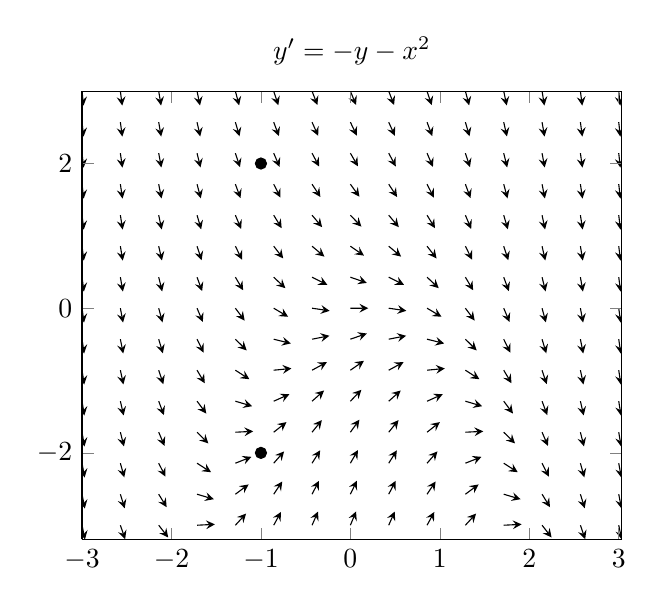
\begin{tikzpicture}
    \begin{axis}[
        title={\(y' = -y -x^2 \)},
        domain=-3:3,
        view={0}{90},
        axis background/.style={fill=white},
    ]
        \addplot3[black,
            quiver={
             u={1/(sqrt(1 + (-y -x*x)^2))},
             v={(-y - x*x)/(sqrt(1 + (-y - x*x)^2))},
             scale arrows=0.2,
            },
            -stealth,samples=15]
                {exp(-x) - 1/2*sin(x) - 1/2*cos(x)};
        %KAWWWWWWW
        % Here be some points added to the swoopy loop vector fieldamagigs
        \addplot[mark=*] coordinates {(-1,2)}; % Obvious ordered pair for lococation
        \addplot[mark=*] coordinates {(-1,-2)};
    \end{axis}
\end{tikzpicture}\end{center}
\end{problem}


\begin{solution}

\begin{center}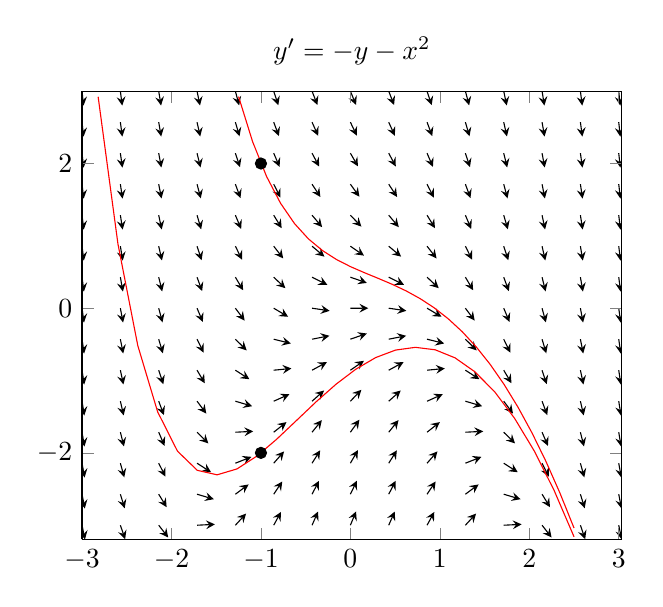
\begin{tikzpicture}
    \begin{axis}[
        title={\(y' = -y - x^2\)},
        domain=-3:3,
        view={0}{90},
        axis background/.style={fill=white},
    ]
        \addplot3[black,
            quiver={
             u={1/(sqrt(1 + (-y -x*x)^2))},
             v={(-y - x*x)/(sqrt(1 + (-y - x*x)^2))},
             scale arrows=0.2,
            },
            -stealth,samples=15]
                {exp(-x) - 1/2*sin(x) - 1/2*cos(x)};
        %KAWWWWWWW
        % Here be some points added to the swoopy loop vector fieldamagigs
        \addplot[mark=*] coordinates {(-1,2)}; % Obvious ordered pair for lococation
		\addplot[red,domain=-1.25:2.5] {-x^2+2*x-2+7/exp(1)*exp(-x)};
        \addplot[mark=*] coordinates {(-1,-2)};
		\addplot[red,domain=-2.82:2.5] {-x^2+2*x-2+3/exp(1)*exp(-x)};
    \end{axis}
\end{tikzpicture}\end{center}
\end{solution}


\begin{problem}{F2}
Solve \(y'+xy=x\).
\end{problem}
\begin{solution}
Rearranging, we have \(y'=x-xy=x(1-y)\), so we see the equation is separable, and write
\[ \frac{y'}{1-y} = x .\]

Thus we compute \(\int \frac{y'}{1-y}\ dx = \int \frac{1}{1-y}\ dy = -\ln|1-y|+c_1\), and \(\int x\ dx = \frac{1}{2}x^2+c_2\).  
Thus, we have (letting \(c_3=c_2-c_1\)) \[-\ln|1-y|=\frac{1}{2}x^2+c_3.\]
Then exponentiating, we have (letting \(c_4=\pm e^{-c_3}\) ) \(1-y=c_4e^{-\frac{1}{2}x^2}\), so (with \(c=-c_4\) ) the general solution is   \[y=1+c e^{-\frac{1}{2}x^2}.\]
\end{solution}

\begin{problem}{F3}
A ball has a mass of \(0.1 {\rm kg}\) and a drag coefficient of \(0.001 {\rm kg/m}\).  It is thrown with a velocity of \(20 {\rm m/s}\). 
\begin{enumerate}[(a)]
\item Write down an IVP modelling the horizontal velocity of the ball (ignore any vertical movement in the ball).
\item How long does it take the ball to travel \(20 {\rm m}\)?
\end{enumerate}
\end{problem}
\begin{solution}
The only force acting on the ball is air resistance (drag), so we have
\[mv'=-bv^2.\]
Substituting in our constants (and dividing through by \(m\)), we have
\[v'=- 0.1v^2 .\]
The initial condition is that it is travelling \(20 {\rm m/s}\), i.e. \(v(0)=20\), giving the IVP 
\[v'=- 0.1v^2 \hspace{5em} v(0)=20.\]
Solving this separable ODE, we obtain \(v=\frac{20}{1+2t}\).  To model the position of the ball, we integrate again, obtaining \(x=\int \frac{20}{1+2t}\ dt = 10 \ln |1+2t| +C\); using \(x(0)=0\), we see \(C=0\).  Then we simply need to solve \(x(t)=20\), i.e. \(20=10\ln|1+2t|\), so \(t=\frac{1}{2}(e^2-1) \approx 3.19 {\rm s}\).
\end{solution}



\begin{problem}{F4}
Consider the autonomous equation 
\[\frac{dx}{dt} = x^2-1.\]  
\begin{enumerate}[(a)]
\item Find and classify the critical points.
\item Describe the long term behavior of the solution passing through the point \( x(4)=0 \).
\end{enumerate}
\end{problem}
\begin{solution}

Note that \(x^2-1=(x-1)(x+1)\), so there are equillibria solutions at \(x=1\) and \(x=-1\).  We can thus compute a number line for \(x'\):

\begin{center}
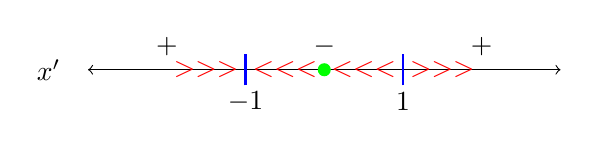
\begin{tikzpicture}
\node at (-3.5,0) {\(x'\)};
\draw[<->] (-3,0) -- (3,0);
\node at (-2,0.3) {\(+\)};
\node at (0,0.3) {\(-\)};
\node at (2,0.3) {\(+\)};
\draw[thick,blue] (-1,-0.2) -- (-1,0.2);
\node at (-1,-0.4) {\(-1\)};
\draw[thick,blue] (1,-0.2) -- (1,0.2);
\node at (1,-0.4) {\(1\)};
\node[red] at (-1.5,0) {\(>>>\)};
\node[red] at (-0.5,0) {\(<<<\)};
\node[red] at (0.5,0) {\(<<<\)};
\node[red] at (1.5,0) {\(>>>\)};
\node[fill,circle,green,scale=0.5] at (0,0) {};
\end{tikzpicture}
\end{center}

We see that \(-1\) is a sink (stable), while \(1\) is a source (unstable).  A trajectory passing through \(x(4)=0\) will approach \(x=-1\) in the limit.
\end{solution}

\begin{problem}{F5}
Solve \(y'+xy=x^3\).
\end{problem}
\begin{solution}
First, we solve the homogeneous equation \(y'+xy=0\), which is separable: \(\frac{y'}{y}=-x\), so \(\ln|y|=-\frac{1}{2}x^2+c\), or \(y=c_1e^{-\frac{1}{2}x^2}\). We then use variation of parameters to find a particular solution, writing \(y_p = v e^{-\frac{1}{2}x^2}\); substituting in and simplifying yields
\[x^3 = y_p ' +xy_p = v'e^{-\frac{1}{2}x^2} -vxe^{-\frac{1}{2}x^2} + xve^{-\frac{1}{2}x^2} = v'e^{-\frac{1}{2}x^2}.\]
Thus, \(v'=x^3 e^{\frac{1}{2}x^2} \).  This can be integrated by parts to obtain \(v=x^2e^{\frac{1}{2}x^2}-2e^{\frac{1}{2}x^2}\), so \(y_p = v e^{-\frac{1}{2}x^2} = x^2-2\).  Thus the general solution is
\[y=c_1e^{-\frac{1}{2}x^2} + x^2 - 2 .\]
\end{solution}

\begin{problem}{F6}
One of the two ODEs below is exact.  Identify which one, and solve it.
\begin{align*}
 (x + 3y)y'+y &=3x \\ %Exact
 (x + 3y)y'-y &=-3x  
\end{align*}
\end{problem}
\begin{solution}
Rewrite the first equation as \(y'=\frac{3x-y}{x+3y}\); if there is a function with \(\nabla F = \langle -(3x-y), x+3y\rangle\), then \[\frac{d}{dt}F(x,y)=\frac{\partial F}{\partial x} \frac{\partial x}{\partial t} + \frac{\partial F}{\partial y} \frac{\partial y}{\partial t} = -(3x-y)(x+3y)+(x+3y)(3x-y)=0,\] so \(F(x,y)=c\) is a solution of the autonomous system.

Note that  \(\langle -(3x-y), x+3y\rangle\) is conservative, as \(\frac{\partial}{\partial x}(x+3y)=1=\frac{\partial}{\partial y}(-3x+y)\); so a potential function \(F\) is found by integrating: \(F = \int x+3y\ dy = xy+\frac{3}{2}y^2+f(x) \), and differentiating with respect to \(x\), we have \(-3x+y=y+f'(x)\), so \(f'(x)=-3x\), in which case \(f(x)=\int -3x\ dx = \frac{-3}{2}x^2\), so a potential function is \(F(x,y)=xy+\frac{3}{2}y^2-\frac{3}{2}x^2\).  So the general solution to the ODE is
\[ xy+\frac{3}{2}y^2-\frac{3}{2}x^2 = c.\]
\end{solution}

\begin{problem}{S1}
Find the general solution of the system
\begin{align*}
x' & = 2x + y,\\
y' & = x + 2y
\end{align*}
\end{problem}
\begin{solution}

We begin by moving all \(x\) and \(y\) terms to one side, and rewriting in terms of differential operators
\begin{align*}
(D-2I)x-Iy & =0 ,\\
(-I)x+(D-2I)y & = 0
\end{align*}
Applying \(D-2I\) to the top equation and adding, we obtain \( (D-2I)^2x-Ix=0\), or \((D^2-4D+3I)x=0\), which factors as \((D-3I)(D-I)x=0\).  Thus the general solution for \(x\) is \(x=c_1 e^{3t}+c_2e^t\).  But rearranging the first equation, we have \(y=x'-2x\), so \(y=\left(c_1 e^{3t}+c_2e^t\right)'-2\left(c_1 e^{3t}+c_2e^t\right) = c_1e^{3t}-c_2e^t\).  Thus the general solution is
\begin{align*}
x&=c_1e^{3t}+c_2e^t \\
y&=c_1e^{3t}-c_2e^t
\end{align*}

\end{solution}

\begin{problem}{S2}
Two populations of competing species of fish, bluegills and greenfish, are modelled by the system
\begin{alignat*}{2}
\frac{dG}{dt} &= 0.1G - 0.005G^2 - 0.004BG \\
\frac{dB}{dt} & = 0.2B - 0.01B^2 - 0.004BG.
\end{alignat*}
\begin{enumerate}[(a)]
\item Identify all equillibrium points for the system.
\item If a lake is stocked with \(25\) bluegills and \(35\) greenfish , what will happen to the two populations in the long term?
\end{enumerate}
\end{problem}
\begin{solution}

The greenfish isocline is given by \[0=0.1G-0.005G^2-0.004BG=0.001G(100-5G-4B)\], while the bluegill isocline is given by 
\[0=0.2B-0.01B^2-0.004BG=0.001B(200-10B-4G).\]

If \(G=0\), then the bluegill isocline implies \(B=0\) or \(200-10B=0\), i.e. \(B=20\), giving two equillibrium points ( \(B=0,G=0\) and \(B=20,G=0\).  On the other hand, if \(100-5G-4B=0\) and \(B=0\), then we obtain an equillibrum point at \(B=0,G=20\); but if \(100-54G-4B=0\) and  \(200-10B-4G=0\), solving this system yields  \( B=2.94, G=17.65\) as an equillibrium point.


Now that we have identified the four equillbrium points, to answer part (b), we plot the isoclines, and the general direction of the slopes in each of the four regions

\begin{center}
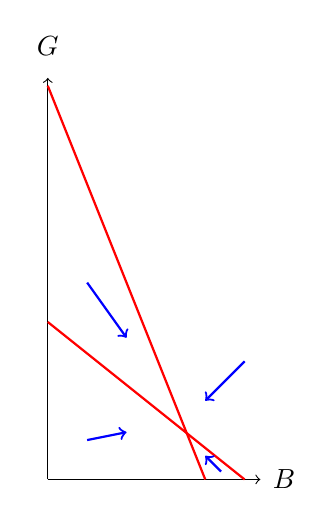
\begin{tikzpicture}[scale=0.1]
\draw[->] (0,0) -- (27,0);
\draw[->] (0,0) -- (0,51);
\node at (30,0){\(B\)};
\node at (0,55){\(G\)};
\draw[thick,red] (25,0) -- (0,20);
\draw[thick,red] (20,0) -- (0,50);
\draw[thick,blue,->] (5,25) -- (10,18);
\draw[thick,blue,->] (5,5) -- (10,6);
\draw[thick,blue,->] (22,1) -- (20,3);
\draw[thick,blue,->] (25,15) -- (20,10);
\end{tikzpicture}
\end{center}

Analyzing the slopes in each of the four regions on the graph shows that the central equillibrium point is a sink.  Thus, in the long term the populations will approach the central equillbirum of \(2.94\) bluegills and \(17.65\) greenfish.

Here is a slope field to make the intuition of the above rough sketch more clear:
\begin{center}
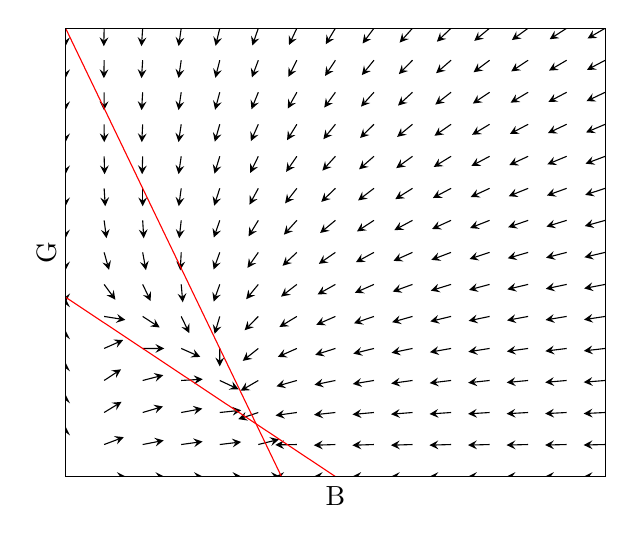
\begin{tikzpicture}
    \begin{axis}[
        domain=0:50,
        view={0}{90},
        axis background/.style={fill=white},
		yticklabels={,,},
		xticklabels={,,},
		xlabel={B},
		ylabel={G},
		ticks=none,
    ]
        \addplot3[black,
            quiver={
             u={10*(0.2*x-0.01*x^2-0.004*x*y)/sqrt(  (0.2*x-0.01*x^2-0.004*x*y)^2+  (0.1*y-0.005*y^2-0.004*x*y)^2)  },
             v={10*(0.1*y-0.005*y^2-0.004*x*y)/sqrt(  (0.2*x-0.01*x^2-0.004*x*y)^2+  (0.1*y-0.005*y^2-0.004*x*y)^2)},
             scale arrows=0.2,
            },
            -stealth,samples=15]
                {exp(-x) - 1/2*sin(x) - 1/2*cos(x)};
		\addplot[red] coordinates {(25,0) (0,20)};
		\addplot[red] coordinates {(20,0) (0,50)};
    \end{axis}

\end{tikzpicture}
\end{center}

\end{solution}

\begin{problem}{S3}
\begin{minipage}[t]{0.8\linewidth}
Consider the dual mass-spring system at the right.  The upper mass is \(2 {\rm kg}\) while the lower is \(1 {\rm kg}\).  The upper spring has a spring constant of \( 2 {\rm N/m}\) while the lower spring constant is \(1 {\rm N/m}\).  The lower spring is pulled down \(1 {\rm m}\) without disturbing the upper spring, and released from rest. 
\begin{enumerate}[(a)]
\item Write down an IVP modelling the motion of the two masses.
\item Where will the two masses be after \(2 {\rm s}\)?
\end{enumerate}
\end{minipage}
\hfill
\springdoublemassQuiz[0.7]
\hfill
\end{problem}
\begin{solution}
Let \(y_1, y_2\) represent the positions of the two masses respectively, as measured from equillibrium.  The lower mass is only affected by the lower spring, so its motion is modelled by \( y_2''=-1(y_2-y_1)\), since the length the lower string is stretched is \(y_2-y_1\).  The upper mass is affected by both springs, so it has a force of \(1(y_2-y_1) \) from the lower spring, and \(-2 y_1\) for the upper spring.  Thus, the upper mass's motion is modelled by \(2y_1''=-2(y_1) + 1(y_2-y_1)\).  Simplifying and adding in the initial conditions \(y_1(0)=0, y_1'(0)=0, y_2(0)=-1, y_2'(0)=0\), we have the IVP
\begin{align*}
2y_1''&=-3y_1+y_2 & y_1(0)=0, y_1'(0)=0 \\
y_2''&= y_1-y_2 & y_2(0)=-1, y_2'(0)=0
\end{align*}

To answer part (b), we need to solve this system.  First, we rewrite in terms of differential operators:
\begin{align*}
(2D^2+3)y_1-y_2 &= 0 \\
-y_1 + (D^2+1)y_2 &= 0\\
\end{align*}

Applying \(D^2+1\) to the top  equation and adding to the bottom yields
\[0=\left( (D^2+1)(2D^2+3) -1 \right)y_1 = (2D^4+5D^2+2)y_1 = (2D^2+1)(D^2+2)y_1\]

Note that the kernel of \(2D^2+1\) is \(c_1 \cos\left(\frac{t}{\sqrt{2}}\right)+c_2 \sin\left(\frac{t}{\sqrt{2}}\right)\) and the kernel of \(D^2+2\) is \(c_3 \cos\left(t\sqrt{2}\right)+c_4 \sin\left(t\sqrt{2}\right)\).  Thus, the general solution for \(y_1\) is 
\[y_1 = c_1 \cos\left(\frac{t}{\sqrt{2}}\right)+c_2 \sin\left(\frac{t}{\sqrt{2}}\right)+c_3 \cos\left(t\sqrt{2}\right)+c_4 \sin\left(t\sqrt{2}\right).\]

Since \(y_2=2y_1''+3y_1\), we thus obtain
\[ y_2 = \frac{1}{2}c_1 \cos\left(\frac{t}{\sqrt{2}}\right)+\frac{1}{2}c_2 \sin\left(\frac{t}{\sqrt{2}}\right)-2c_3 \cos\left(t\sqrt{2}\right)-2c_4 \sin\left(t\sqrt{2}\right).\]

Now, using our initial conditions, we have
\begin{align*}
0 &= y_1(0) = c_1+c_3 \\
-1 &= y_2 (0) = \frac{1}{2}c_1-2c_3 \\
0 &= y_1'(0) = \frac{1}{\sqrt{2}}c_2+\sqrt{2}c_4 \\
0 &= y_2'(0) = \frac{1}{2\sqrt{2}} c_2 -2\sqrt{2}c_4
\end{align*}

The last two equations imply \(c_2=c_4=0\), while the first two yield \(c_1=-\frac{2}{5}\) and \(c_3 = \frac{2}{5}\).  Thus, the solution to the IVP is
\begin{align*}
y_1 &= -\frac{2}{5} \cos\left(\frac{t}{\sqrt{2}}\right)+\frac{2}{5}\cos\left(t\sqrt{2}\right) \\
y_2 &= \frac{1}{5} \cos\left(\frac{t}{\sqrt{2}}\right)-\frac{4}{5} \cos\left(t\sqrt{2}\right)
\end{align*}

Thus, after two seconds, the upper mass is at \(y_1(2) \approx -0.443\) (i.e. \(0.443 {\rm m}\) down) and the lower mass is at \(y_2(2) \approx 0.792\) (i.e. \(0.792 {\rm m}\) up).
\end{solution}


\begin{problem}{N1}

\end{problem}
\begin{solution}

\end{solution}

\begin{problem}{N2}

\end{problem}
\begin{solution}

\end{solution}

\begin{problem}{N3}

\end{problem}
\begin{solution}

\end{solution}

\begin{problem}{N4}

\end{problem}
\begin{solution}

\end{solution}

\begin{problem}{N5}

\end{problem}
\begin{solution}

\end{solution}


\begin{problem}{D1}

\end{problem}
\begin{solution}

\end{solution}

\begin{problem}{D2}

\end{problem}
\begin{solution}

\end{solution}

\begin{problem}{D3}

\end{problem}
\begin{solution}

\end{solution}

\begin{problem}{D4}

\end{problem}
\begin{solution}

\end{solution}



\end{document}
